\documentclass[a4paper,11pt]{report}

\usepackage{keyval}
\usepackage[T1]{fontenc}
\usepackage[utf8]{inputenc}
\usepackage[italian]{babel}
\usepackage{graphicx}
\usepackage{geometry}
\usepackage{xcolor}
\usepackage[hidelinks, pdfhighlight = /N]{hyperref}
\usepackage{bookmark}
\usepackage{longtable}
\usepackage{listingsutf8}
\usepackage{color, colortbl}
\usepackage{hyperref}
\usepackage{ragged2e}
\usepackage{blindtext}
\usepackage{float}

\definecolor{dkgreen}{rgb}{0,0.6,0}
\definecolor{gray}{rgb}{0.5,0.5,0.5}
\definecolor{mauve}{rgb}{0.58,0,0.82}

\lstset{language=SQL,
  inputencoding=utf8,
  literate = {à}{{\ `a}}2 {À}{{\`A}}1 
  			 {ò}{{\ `o}}2 {Ò}{{\`O}}1 
			 {è}{{\ è}}2 {È}{{\`E}}1 
			 {ù}{{\ `u}}2 {Ù}{{\`U}}1,
  extendedchars=true,
  basicstyle={\normalsize\ttfamily},
  belowskip=3mm,
  breaklines=true,
  classoffset=0,
  columns=flexible,
  commentstyle=\color{dkgreen},
  framexleftmargin=0em,
  frameshape={}{yy}{}{}, %To remove to vertical lines on left, set frameshape={}{}{}{}
  keywordstyle=\color{blue},
  numbers=left, %If you want line numbers, set numbers=left
  numberstyle=\normalsize\color{gray},
  showstringspaces=false,
  stringstyle=\color{mauve},
  tabsize=3,
  xleftmargin =5pt,
}

\justifying

\begin{document}

	\begin{titlepage}

\begin{figure} [h]
\vspace{-2cm}
\hspace{-20mm}
%\includegraphics[scale=0.35]{Logo unina}
\end{figure}
\vspace{2mm}

\begin{center}
\Large {CORSO DI LAUREA IN INFORMATICA\\
\centering INSEGNAMENTO DI LABORATORIO DI SISTEMI OPERATIVI \\
ANNO ACCADEMICO 2021/2022\\}
\end{center}
\vspace{10mm}

\begin{center}{
\Huge \textbf {Progettazione di un applicazione\\ per la rilevazione\\\vspace{2mm} di buche su strada}}
\end{center}
\vspace{4cm}

\begin{flushleft}
{\large \textbf {STUDENTI}  \\
\vspace{2mm}
Caccavale Mariano  N86003303 \\ 
mariano.caccavale@studenti.unina.it\\
\vspace{3mm}
Rossi Mattia N86003211 \\
matti.rossi@studenti.unina.it\\}
\end{flushleft}

\vspace{-42mm}
\hspace{4cm}
\begin{flushright}
{\large \textbf {PROFESSORI} \\
\vspace{2mm}
Grazioso Marco \\ marco.grazioso@unina.it\\
\vspace{3mm}
Scala Giovanni \\  giovanni.scala@unina.it\\}
\end{flushright}

	\end{titlepage}
	\clearpage

\thispagestyle{empty}
\centering
 \, \\  \, \\ \, \\ \, \\ \, \\ \, \\ \, \\ \, \\ \, \\ \, \\ \, \\ \, \\ \, \\ \, \\ \, \\ \, \\ \, \\ \, \\ \, \\ \, \\ \, \\ \, \\ \, \\ \, \\ \, \\ \, \\ \, \\ \, \\ 
 
 {\huge\emph{Questa documentazione è stata scritta in Latex}}

\clearpage


	\newgeometry{tmargin = 0.2in, bmargin = 0.8in}
	\tableofcontents
	\newgeometry{tmargin = 1.5cm, bmargin = 0.8in}
	\chapter{\Large{\textbf{Descrizione del progetto}}}
\justifying
\vspace{-10mm}
\section{\large{\textbf{Traccia del progetto}}}

Il sistema deve memorizzare e rendere disponibile una lista di eventi generati dai clients riguardanti la rilevazione di una un repentino cambiamento dell' accelerazione lungo l' asse verticale che superi una soglia comunicata dal server in fase di connessione. Ciascun client è identificato da un nickname, scelto dall' utente.
Il sistema tramite il client deve offrire agli utenti i seguenti servizi: \newline
 1) Permettere all' utente di avviare una sessione di registrazione eventi durante la quale il client si connette al server, riceve i parametri di soglia e comunica al server la posizione e il valore del cambiamento ogni volta che registra un nuovo evento. \newline
2) Mostrare all' utente la lista di tutti gli eventi registrati dal server in un certo raggio dalla propria posizione. 
\justifying


\justifying
\noindent

\section{\large{\textbf{Guida al Client}}}
Il client della nostra applicazione è stato reso lineare per facilitare i nuovi utenti all'uso immediato dell'app.\newline
La prima schermata che si presenta all'utente ad ogni apertura dell'app è composta da un messaggio di benvenuto e la richiesta all'inserimento di un nickname.\newline 

\begin{figure} [H]
\centering
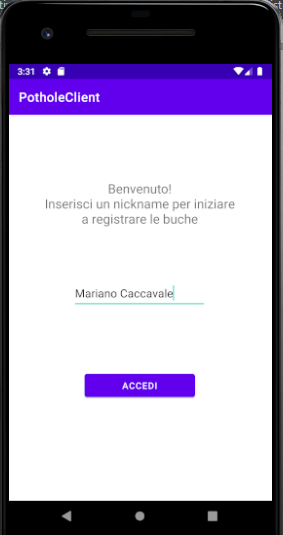
\includegraphics[scale=0.65]{login_screen}
\caption{Schermata di apertura}
\end{figure}
\newpage

Dopo aver digitato un nickname valido e premuto il tasto accedi si passa alla schermata principale dell'app dove si presenta un breve menù dove l'utente può selezionare la funzione da svolgere.\newline  
\begin{figure} [H]
\centering
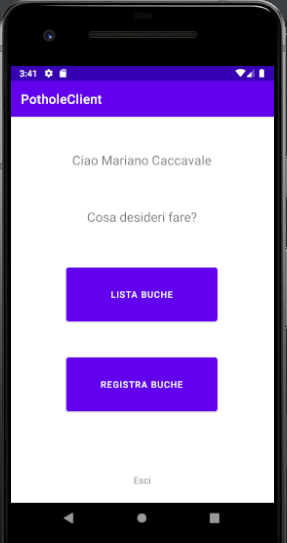
\includegraphics[scale = 0.65]{menu_screen}
\caption{Schermata principale}
\end{figure}


Nel caso si scelga la funzione di registra buche, si aprirà una schermata dove verrà chiesto al client di calibrare il dispositivo per iniziare a registrare, dove veranno usati valori di treshold passati dal server al client.
\begin{figure} [H]
\centering
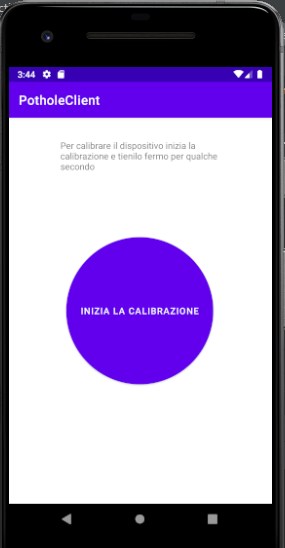
\includegraphics[scale = 0.65]{start_calibration_screen}
\caption{Apertura della funzione di registrazione}
\end{figure}

\newpage 
Dopo che l'app abbia calibrato il dispositivo con successo, l'utente può iniziare la sessione di registrazione premendo sul pulsante di start.\newline
\begin{figure} [H]
\centering
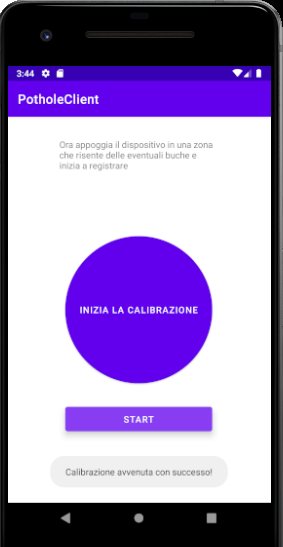
\includegraphics[scale = 0.65]{start_recording_screen}
\caption{Apertura della funzione di registrazione}
\end{figure}


Nel caso l'app rilevi una buca verrà visualizzato un piccolo messaggio di avviso per l'utente.
\begin{figure} [H]
\centering
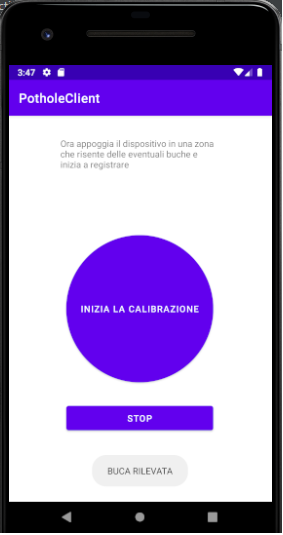
\includegraphics[scale = 0.65]{potholes_detected}
\caption{Rilevazione di una buca}
\end{figure}
\newpage
L'altra funzionalità dell'app è invece la visualizzazione delle buche in un range prefissato dalla posizione del client, questo può dare due possibile risoluzioni della richiesta: 

\begin{figure} [H]
\centering
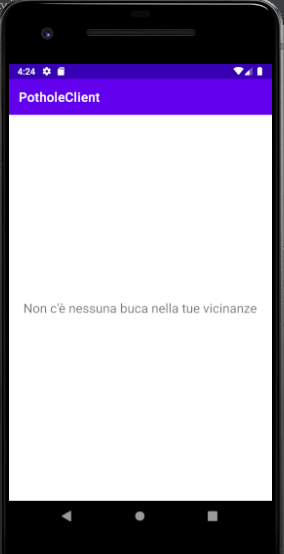
\includegraphics[scale = 0.65]{empty_potholes_list}
\caption{Nessuna buca nelle vicinanze}
\end{figure}


\begin{figure} [H]
\centering
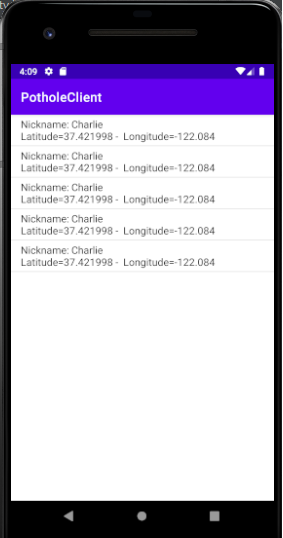
\includegraphics[scale = 0.67]{potholes_list}
\caption{Lista di buche nelle vicinanze}
\end{figure}
\newpage
\section{\large{\textbf{Guida al Server}}}
Il codice del Server (utilizzabile solo su piattaforma Linux) è composto da due cartelle: Client-Server e Database. \newline
Nella prima sono presenti 5 file: initServer.c e initServer.out rispettivamente il codice sorgente e l'eseguibile della prima apertura del Server con creazione (nel caso non sia presente) del database nominato potholes.db. Gli ultimi due file sono server.c e server.out che, come i due file di initServer, sono di codice e di esecuzione del server dalla seconda volta di utilizzo.\newline
Mentre nella cartella Database è presente il file sql.c e il suo relativo backup; tale file è una libreria fatta ad hoc utilizzata nel codice del server per l'interazione tra, appunto, il server e il database.
Se il server viene aperto per la prima volta su un dispositivo, è necessario far eseguire il file initServer.out dove nel caso di corretta esecuzione creera il database contenente la tabella di registrazione delle buche incontrate dagli utenti. Dalla seconda esecuzione.


\newpage


\chapter{\Large{\textbf{Protocollo applicativo}}}

Abbiamo preferito l'uso del protocollo TCP a quello UDP per la presenza di controllo della congestione e affidabilità in termini di consegna messaggi. Per la creazione del protocollo siamo partiti dal Server, in quanto volevamo gettare la basi della comunicazione partendo dalla parte che ascoltasse. \newline
Per via della loro semplicità in C, il Server gestisce le richieste dei Client attraverso Threads, poichè ciò permette al Server di servire diverse richieste in modo concorrente, senza però smettere di ascoltare le connessioni in entrata. Di conseguenza anche il Client adotta un sistema di networking che sfrutta i Threads, considerando anche, ma non solo, l'impossibilità di eseguire operazioni di networking sul Main Thread.\newline
La prima connessione tra Client e Server avviene dopo l'inserimento del nickname, dove il Client manda richiesta al Server di ricevere valori di tolleranza (usati durante la sessione di registrazione buche). Delle tre richieste che il Client fa al Server l'unica diversa è l'acquisizione di buche, dove il Client crea una connessione con il server non all'inizio della sessione di registrazione, ma solo dopo il rilevamento di una buca per impedire che possono avvenire timeout improvvisi durante la registrazione delle buche. 
\newpage


\chapter{\Large{\textbf{Dettagli implementativi}}}
La panoramica sui dettagli implementativi si suddivide in due sezioni: La prima riguarda il codice del Server, con un occhio di riguardo alle system call usate, mentre la seconda ricopre il codice del lato Client e la classe usata per la connessione Client-Server.

\section{\Large{\textbf{Lato Server}}}
Questo estratto del codice racchiude tutte le system call usate più importanti, quali: 

\begin{itemize}
\item signal: ci permette di definire un handler per una specifica tipologia di segnale.
\item socket: creazione dell'oggetto di tipo socket.
\item bind: funzione che assegna ad una socket le informazioni a corredo.
\item listen: funzione che permette ad una socket di ascoltare attivamente.
\item accept: funzione che accetta le connessioni in entrata.
\item pthreadcreate: funzione che assegna alla struttura thread una funzione e la esegue.
\end{itemize}

\subsection{connessione}

\begin{lstlisting} [language = C]
//Dichiaro l'handler del segnale USR1, in modo da avere un modo 'safe' di chiudere il server
    signal(SIGUSR2,signUSRHandlet); 

    int clientSocket, new_sock;

    //Struttura dati sockets
    struct sockaddr_in server , client;

    char hostname = "0.0.0.0";

    if( ( socketDescriptor = socket(AF_INET, SOCK_STREAM, 0) ) < 0 ){

        perror("Errore nella creazione della socket\n");
        exit(1);

    }

    //Assegno i valori alla struttura 'server'
    server.sin_family = AF_INET;
    server.sin_addr.s_addr = inet_addr(hostname);
    server.sin_port = htons(PORT_N);


    //Avverto il sistema operativo che voglio che la socket sia 'riconosciuta' e entri in funzione
    if( ( bind(socketDescriptor, (struct sockaddr) &server, sizeof(server)) ) < 0 ){

        perror("Errore nel binding\n");
        exit(1);

    }

    printf("[] Binding effettuato con successo\n");

  listen(socketDescriptor, 10);

    printf("[] Sono in ascolto su %s : %d. Attendo nuove connessioni...\n", hostname, PORT_N);

    int c = sizeof(struct sockaddr_in);


    while( (clientSocket = accept(socketDescriptor, (struct sockaddr)&clientSocket, (socklen_t*)&c) ) > 0){

if( pthread_create(&thread, NULL, threadFunction, (void*) new_sock) < 0 ){

            perror("Errore nella creazione di un thread\n");

        }

void signUSRHandlet(int signal){

    printf("[] Ricevuto segnale USR, procedo alla chiusura del server.\n");
    close(socketDescriptor);
    printf("[] Server out!\n");
    exit(0);

}
   
\end{lstlisting}

\subsection{getTolerance}
Snippet di codice che viene eseguito se il Server rileva la richiesta della tolleranza da parte del Client.
\begin{lstlisting} [language = C]
else if(strcmp(requestBuffer, "toll") == 0){

                send(socketDesc, "0.000002;", 8, 0);

        }
\end{lstlisting} 

\subsection{sendData}
Lettura dei dati inviati dal Client con successivo inserimento degli stessi all'interno del Database.
\begin{lstlisting} [language = C]
oid postRequest(int socketDescriptor){

    char readBuffer[1000];
    int byteLetti = 0, byteScritti = 0;

    //Riferimento al database in cui andrò ad inserire i dati
    sqlite3* database;

    //Leggo fin quando ha dati da mandarmi
    recv(socketDescriptor, readBuffer, 2000, 0);
    //printf("%s\n", readBuffer);


    char* field = strtok(readBuffer, ";");
    char nickname[20];
    char latitude[20];
    char longitude[20];
    int charN = 0;

    while(field != NULL){

        if(charN == 0){
            strcpy(nickname, field);
        }else if (charN == 1){
            strcpy(latitude, field);
        }else if (charN == 2){
            strcpy(longitude, field);
        }
        charN++;

        field = strtok(NULL, ";");

    }

    //Chiedo alla funzione di aprire il database chiamato 'potholes'
    int status = sqlite3_open_v2("potholes.db", &database, SQLITE_OPEN_READWRITE | SQLITE_OPEN_NOMUTEX, NULL);

    if(status == SQLITE_OK){

        status = insertPothole(database, nickname, atof(latitude), atof(longitude));

        if(status == SQLITE_OK){

            printf("[*] Inserimento avvenuto con successo\n");

        }else{

            printf("[!] Inserimento fallito - %d\n", status);

        }

    }else{

        printf("[!] Apertura del database fallita\n");

    }

    //Mi congedo da client
    printf("[*] Comunicazione terminata, chiudo la connessione\n");

    sqlite3_close(database);

    return;

}
\end{lstlisting}

\subsection{receiveData}
Interrogazione che il Server esegue sul Database data la posizione di un Client e conseguente invio dellla eventuale lista di buche eseguito dalla funzione getPotholes in un range fissato dal Server.

\begin{lstlisting} [language = C]

void getRequest(int socketDescriptor){

    char readBuffer[1000];
    int byteLetti = 0, byteScritti = 0;

    //Riferimento al database in cui andrò ad inserire i dati
    sqlite3* database;

    //Leggo fin quando ha dati da mandarmi
    recv(socketDescriptor, readBuffer, 2000, 0);
    //printf("%s\n", readBuffer);


    char* field = strtok(readBuffer, ";");
    char nickname[20];
    char latitude[20];
    char longitude[20];
    int charN = 0;

    while(field != NULL){

        if(charN == 0){
            strcpy(nickname, field);
        }else if (charN == 1){
            strcpy(latitude, field);
        }else if (charN == 2){
            strcpy(longitude, field);
        }
        charN++;

        field = strtok(NULL, ";");

    }

    printf("Dati su cui sto andando a fare la ricerca: %s - %f - %f\n", nickname, atof(latitude), atof(longitude));

    //Chiedo alla funzione di aprire il database chiamato 'potholes'
    int status = sqlite3_open_v2("potholes.db", &database, SQLITE_OPEN_READWRITE | SQLITE_OPEN_NOMUTEX, NULL);

    if(status == SQLITE_OK){

        status = getPotholes(database, atof(latitude), atof(longitude), socketDescriptor);

        if(status == SQLITE_OK){

            printf("[*] Ricerca avvenuta con successo\n");

        }else{

            printf("[!] Ricerca fallita - %d\n", status);

        }

    }else{

        printf("[!] Apertura del database fallita\n");

    }

    //Mi congedo da client
    printf("[*] Comunicazione terminata, chiudo la connessione\n");

    sqlite3_close(database);

    return;

}

\end{lstlisting}


\section{\Large{\textbf{Lato Client}}}

\subsection{Lato Client}
Funzione che viene invocata dall'utente per ricevere una lista di buche nelle sue vicinanze. 

\begin{lstlisting} [language =  Java]
public static LinkedList<PotholesModel> receiveData(String myNickname, double myLatitude, double myLongitude){

        LinkedList<PotholesModel> resultList = new LinkedList<>();

        try {
            Socket socket = new Socket(Costants.ip, Costants.port);

            String get = "get";
            socket.getOutputStream().write(get.getBytes());

            BufferedReader stdIn =
                    new BufferedReader(
                            new InputStreamReader(socket.getInputStream()));

            String dati = myNickname+";"+myLatitude+";"+myLongitude;
            socket.getOutputStream().write(dati.getBytes());

            Thread.sleep(500);

            String responseBuffer;
            while(stdIn.ready()){
                responseBuffer = stdIn.readLine();
                responseBuffer = responseBuffer.replace("\u0000", "");
                if(responseBuffer.isEmpty()){
                    break;
                }
                String[] fields = responseBuffer.split(";");
                String nickname = fields[0];
                double latitude = Double.parseDouble(fields[1]);
                double longitude = Double.parseDouble(fields[2]);

                resultList.add(new PotholesModel(nickname, latitude, longitude));

            }
        } catch (IOException | InterruptedException e) {
            e.printStackTrace();
        }
        return resultList;
    }

\end{lstlisting}

\subsection{Lato Client}
Questa funzione viene invocata da parte del Client subito dopo l'accesso dell'utente per recuperare i valori di tolleranza dal Server.

\begin{lstlisting}[language = Java]
public static double getTolerance(){

        String getTolerance = "toll";
        String toleranceString = "0.000000";

        try {
            Socket socket = new Socket(Costants.ip, Costants.port);
            BufferedReader stdIn =
                    new BufferedReader(
                           new InputStreamReader(socket.getInputStream()));

            socket.getOutputStream().write(getTolerance.getBytes());

            if(stdIn.ready()){
                toleranceString = stdIn.readLine();
                toleranceString = toleranceString.replace("\u0000", "");
                toleranceString = toleranceString.replace(";", "");
            }

            socket.close();

        } catch (IOException e) {
            e.printStackTrace();
        }

        return Double.parseDouble(toleranceString);
    }

\end{lstlisting}


\subsection{Lato Client}
Funzione che viene invocata automaticamente ogni volta che il Client rileva una buca, creando  un messaggio contenente i dati convertiti in formato byte.

\begin{lstlisting} [language =  Java]
public static void sendData(String nickname, double latitude, double longitude){

        //Creo il socket a cui mandare i dati
        try {
            Socket socket = new Socket(Costants.ip, Costants.port);

            //Debug
            //String dati = "Charlie;78.000015;96.369874";

            String post = "post";
            socket.getOutputStream().write(post.getBytes());

            String dati = nickname+";"+latitude+";"+longitude;
            socket.getOutputStream().write(dati.getBytes());

            socket.close();

        } catch (IOException e) {
            e.printStackTrace();
        }
    }

\end{lstlisting}



\end{document}